\documentclass[a4paper,11pt]{article}
\usepackage{amsmath}
\usepackage{polski}
\usepackage[polish]{babel}
\usepackage[utf8]{inputenc}
\usepackage[T1]{fontenc}
\usepackage{graphicx}
\usepackage{anysize}
\usepackage{enumerate}
\usepackage{times}
\usepackage{plain}
\usepackage{caption}
\usepackage{graphicx}

\begin{document}

\begin{figure}[!htb]
	\centerline{
\includegraphics[scale=1]{agh_logo.jpg}}
\end{figure}

\begin{center}
	\Huge{Modelowanie i Symulacja Systemów\\
		Data-driven modelling:\\ Predykcja ruchu samochodów\\}
	\date{}
%	\maketitle

	\vspace{3cm}
	\Large{	Autorzy:\\
		Łukasz Gosek\\
		Fryderyk Muras\\
		Przemysław Michałek\\}

	\newpage

	
\end{center}
\begin{enumerate}
	\item \textbf{{\Large Wprowadzenie}}\\ \\
		\begin{large}
		Zatory komunikacyjne przyciągają uwagę wielu naukowców, ponieważ stają się jednym z największych problemów środowisk miejskich. Aby zrozumieć zjawisko zatłoczenia ruchu, naukowcy przeprowadzili wiele badań na podstawie
różnych modeli i metod. Model automatu komórkowego (Cellular Automaton) opracowany przez Nagela i Schreckenberga \cite{nagel1992cellular} jest jednym z najwydajniejszych modeli problemów z przepływem ruchu.
Przepływ ruchu jest zależny od kilku czynników, w tym od zachowania kierowców (np. niedoskonały styl jazdy, wolniejsze samochody i wypadki), które odgrywają ważną rolę w tworzeniu się korków w systemie transportowym, zwłaszcza w połączeniu ze wzrostem ilości i co za tym idzie gęstości samochodów \cite{chowdhury2000statistical}. Gdy zwiększa się gęstość samochodów zachodzi przejście fazowe: ze swobodnego przepływu do fazy przeciążenia. W fazie swobodnego przepływu samochody poruszają się z prędkością bliską ograniczeniu, co prowadzi do zwiększenia gęstości pojazdów. Jednak faza przeciążenia charakteryzuje się ujemną liniową zależnością między przepływem ruchu a gęstością. Wykazano, że w fazie przeciążenia zachowanie kierowców ma znaczny wpływ na przestrzenną dystrybucję pojazdów na drodze
względem siebie \cite{jarai2012earthquake}.
Jednym z rozwiązań rozładowania zbyt gęstego ruchu drogowego jest rondo - skrzyżowanie bez świateł oferujące rozwiązania
korzystne pod względem bezpieczeństwa obiegu, opóźnień i przepustowości. Zostało po raz pierwszy opracowane w Wielkiej Brytanii i obecnie jest szeroko stosowane w
większości państw. Kierowcy zbliżający się do ronda muszą zmniejszyć prędkość i przed wjazdem szukać potencjalnych konfliktów z pojazdami, które już są na rondzie.\\

W wielu raportach stwierdzono, że ryzyko wypadku na rondach znacznie zmalało
w porównaniu z innymi konwencjonalnymi skrzyżowaniami \cite{persaud2001safety}. Jednak wypadki samochodowe na środku ronda są jednym z najczęstszych czynników przyczyniających się do powstawania zatoru. Wśród przyczyn wypadków samochodowych jest wysoka prędkość i wymuszanie pierwszeństwa. Pomimo wykazanych korzyści bezpieczeństwa rond, wypadki na nich zdarzają się regularnie. Badanie kolizji na 38 rondach w Maryland wykazało, że zdarzały się one częściej
przy wjazdach na ronda niż wewnątrz czy przy wyjściach \cite{mandavilli2009crash}.
		\end{large}


%	\begin{enumerate}
%		\item a
%		\item b
%		\item c
%		\item d 
%	\end{enumerate}

	\newpage
	\item \textbf{{\Large Proponowany model}}\\ \\
	 \begin{large}
			Wspomniane we wprowadzeniu automaty komórkowe można przedstawić w postaci czwórki (L, S, N, f), gdzie kolejne elementy oznaczają: przestrzeń podzieloną na siatkę cel, zbiór skończonych stanów, zbiór sąsiadów danej celi oraz funkcję zmiany konfiguracji w poszczególnych celach. Konfiguracja C:L $\rightarrow$ S jest funkcją, która łączy każdą celę siatki ze stanem. Funkcja f zmienia konfigurację C$_{t}$ w nową konfigurację C$_{t+1}$. O klasyfikacji automatów komórkowych można dowiedzieć się więcej w pracy \cite{wkasalgorytmy} o ich użyciu, również dla predykcji ruchu pieszych, w pracy \cite{wkas2004zastosowanie}, dokonano też w pracy \cite{dudek2005formalizacja} pewnej formalizacji dla automatów ze stałą siatką, wykorzystywanych do modelowania systemów o stałej topologii przestrzennej. Założenia tej pracy będą wykorzystywane w dalszej części projektu.\\ \\
			 Klasycznym modelem opisującym ruch samochodowy (opartym na automatach komórkowych) jest model Nagela-Schreckenberga \cite{nagel1992cellular} (nazywany krócej \textit{Na-Sch}). Model ten z założenia opisuje ruch samochodów na autostradzie, lecz po kilku modyfikacjach można opisać nim również ruch miejski. W modelu \textit{Na-Sch} przyjęty został stały rozmiar komórki równy \textit{d = 7,5} m, w każdej komórce może znajdować się tylko jeden pojazd, prędkość pojazdu opisywana jest liczbą komórek pokonywanych przez pojazd w następnej iteracji. \textit{Na-Sch} opisują następujące reguły ruchu:
			 \begin{itemize}
				\item Przyspieszenie: \textit{v(t + 1)} $\rightarrow$ min( \textit{v(t} + 1), \textit{v}$_{max}$), gdzie \textit{v(t)}	to prędkość aktualna
				\item Hamowanie: \textit{v(t + 1)} $\rightarrow$ min( \textit{v(t} + 1), \textit{g(t)} - 1), gdzie \textit{g(t)}	jest liczbą pustych komórek pomiędzy pojazdami
				\item Element losowy (nieuzasadnione, przypadkowe hamowanie): prawdopodobieństwo \textit{p}, że nastąpi \textit{v(t} + 1) $\rightarrow$ max(\textit{v(t} - 1)), jeżeli \textit{v(t)} >= 1
				\item Ruch: \textit{x(t + 1)} = \textit{x(t)} + \textit{v(t)}
			 \end{itemize}
			
			\begin{figure}[!htb]
				\centering
				\captionsetup{justification=centering,margin=2cm}
				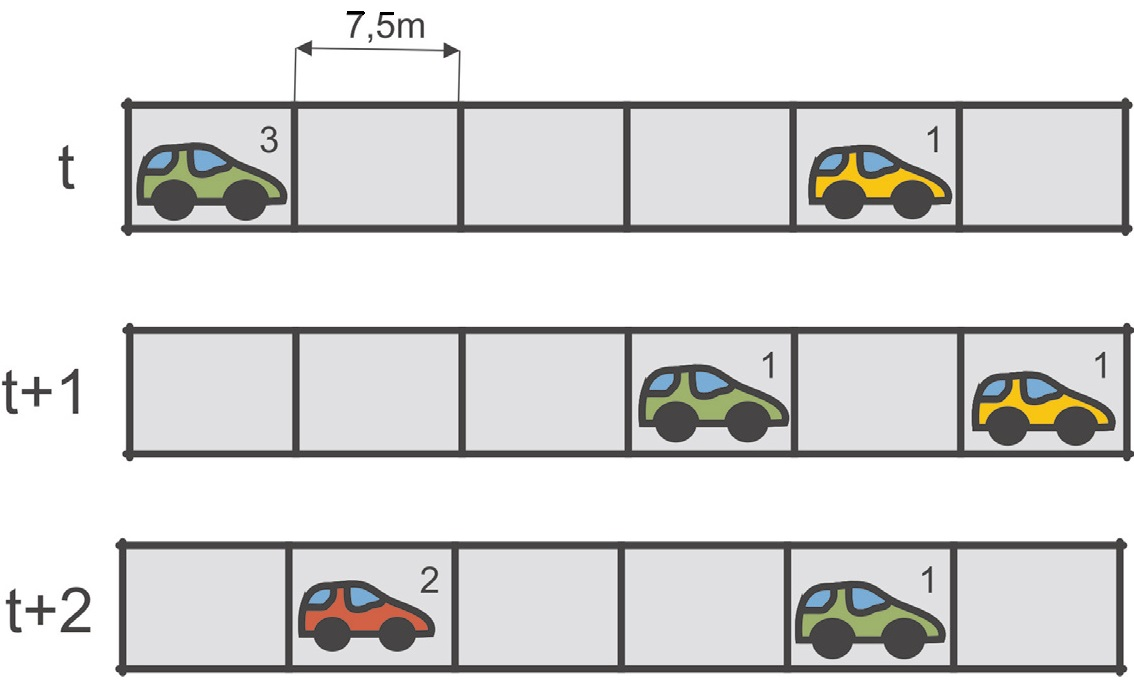
\includegraphics[scale=0.35]{Na-Sch.jpg}

				\caption{Ruch w \textit{Na-Sch} dla jednego pasa ruchu. \\Liczby przy samochodach oznaczają aktualną prędkość pojazdu $\rightarrow$ liczbę pokonywanych komórek w trakcie iteracji}
			\end{figure}
			
	\newpage			
			
			Na bazie modelu \textit{Na-Sch} stworzono z sukcesem szereg wiarygodnych modeli dla ruchu samochodowego o czym świadczy liczba łącznych cytowań (ponad 4 500) artykułu w którym model został opublikowany. Wśród tych prac należy wyróżnić pracę Hartmana \cite{hartman2004head} w której autor wprowadza nie tylko obsługę wielu pasów ruchu jak również ronda, skrzyżowania, uwzględnia długości poszczególnych typów pojazdów (motocykl, samochód, ciężarówka etc) oraz odpowiednio modyfikuje prędkości dla potrzeb realizmu modelu. Bardzo szczegółowo wykorzystanie \textit{Na-Sch} opisuje również praca \cite{regragui2018cellular} gdzie z kolei każde skrzyżowanie zastąpione jest rondem.\\
			
			Głównym powodem dla którego czysty model \textit{Na-Sch} nie gwarantowałby wiarygodnych rezultatów dla ruchu w mieście jest jego pierwotne założenie: ma opisywać ruch na autostradzie. Ruch pojazdów na autostradzie diametralnie różni się od ruchu miejskiego, gdzie pojazdy naprzemiennie przyspieszają i hamują. Niemal każdy samochód porusza się z inną prędkością niż jadący blisko inny pojazd co wymaga innego podejścia. Różnice pomiędzy modelowanym ruchem miejskim a rzeczywistością opisuje książka \cite{wagner1995traffic}. W naszym modelu wprowadzono odpowiednie modyfikacje:
			\begin{itemize}
				\item Przedwczesne unikanie kolizji: zwalnianie przed najbliższym  pojazdem z dużym wyprzedzeniem
				\item Warunki koniecznie do zmiany pasa ruchu: zbliżanie się do poprzedzającego pojazdu oraz wolny pas obok
				\item Szansa niezmienienia pasa ruchu pomimo spełnionego warunku zmiany (losowość zachowania kierowców)
			\end{itemize}
			\end{large}

	%\newpage
	\item \textbf{{\Large Symulacja zjawiska}}\\
	
	\item \textbf{{\Large Wyniki Symulacji}}\\

	\item \textbf{{\Large Wnioski}}\\
	
\end{enumerate}

\newpage


\bibliographystyle{unsrt}
\bibliography{Bibliografia}
\end{document}
